\chapter{Espectroscopía}
La espectroscopía es una de las técnicas fundamentales de la astronomía, ya que permite determinar la composición química de diferentes fuentes astronómicas, sus propiedades físicas, velocidades radiales y distancias. Además, la espectroscopía es la herramienta que se utiliza para determinar la masa de estrellas en sistemas binarios, calcular el contenido de materia oscura en galaxias y descubrir exoplanetas, entre otras cosas. En esta clase abordaremos algunos conceptos de espectroscopía y revisaremos cómo se utilizan para estudiar el cielo. 

\section{Conceptos de espectroscopía}
\subsection{Líneas espectrales}
Comenzaremos definiendo un concepto muy importante en astronomía: un espectro. Llamamos \textbf{espectro} de una fuente a una representación gráfica que muestra cómo varía la intensidad de la luz de dicha fuente en función de su longitud de onda o su frecuencia. En este sentido, la espectroscopía como una técnica que se utiliza para estudiar los espectros de una fuente cuando su luz interactúa con la materia.

En 1666, Isaac Newton demostró que un prisma de vidrio puede dispersar la luz solar en un espectro. Estudios posteriores mostraron que sobre los colores del espectro solar aparecen algunas líneas oscuras. En 1815, Joseph von Fraunhofer obtuvo alrededor de 574 líneas sobre el espectro solar. Debido a esto, ahora son llamadas <<líneas de Fraunhofer>>. En la Figura \ref{fig:solar-spectrum} se muestra un espectro solar con líneas de Fraunhofer. 

\begin{figure}[htb]
  \centering
				
\includegraphics[width=\textwidth]{figures/solar-spectrum.png}
				\caption{Espectro solar con líneas de Fraunhofer. (Fuente: \href{https://bass2000.obspm.fr/solar_spect.php}{BAse de données Solaire Sol.})}
				\label{fig:solar-spectrum} 
\end{figure}

Para comprender qué son estás líneas oscuras, debemos revisar algunos conceptos sencillos de mecánica cuántica.

\subsubsection{Producción de líneas espectrales}
Las líneas espectrales aparecen en dos formas: en espectros de absorción, donde aparecen líneas oscuras en un fondo brillante (como en el caso del espectro solar) y en espectros de emisión, donde aparecen líneas brillantes sobre un fondo oscuro. Ambos tipos de líneas se deben a interacciones cuánticas entre electrones que orbitan a los átomos y fotones de luz. 

Sabemos que los fotones tienen una energía específica que depende de su frecuencia. Esta energía está dada por $ E = h\nu $. En el modelo semi-clásico del átomo, también llamado el átomo de Bohr, un electrón orbita al núcleo en un nivel de energía estable. Este nivel estable es llamado el nivel base, porque es el de menor energía. Si un fotón con una frecuencia especifica interactúa con el electrón, éste puede ganar la energía suficiente para subir a un nivel de energía superior. A este proceso se le llama <<excitación>>, y se dice que el átomo se encuentra en un nivel excitado. Si eso ocurre, entonces el fotón original es absorbido por el electrón de modo que ya no puede ser detectado por un observador. Posteriormente, cuando el electrón se encuentra en un nivel superior, ocurre el proceso de <<desexcitación>> y salta de nuevo hacia un nivel inferior, emitiendo en el proceso un fotón a una frecuencia específica. Sin embargo, este fotón es emitido en una dirección aleatoria, no en la misma dirección que el fotón incidente original. 

Los espectros de absorción ocurren cuando el átomo absorbe fotones y pasa a un estado excitado. Las líneas oscuras son, por lo tanto, los fotones que fueron absorbidos. En cambio, los espectros de emisión ocurren cuando una fuente se encuentra en estado excitado y pasa a un estado de menor energía, liberando fotones. Las líneas brillantes son, por lo tanto, los fotones emitidos. 

Cuando electrones en un átomo de hidrógeno en cualquier nivel $ n > 2 $  realizan una transición al nivel $ n=2 $ se producen líneas de emisión en el rango visible, conocidas como la \textbf{serie de Balmer}. Por ejemplo, cuando la transición ocurre desde $ n=3 $ hasta $ n=2 $, la línea de emisión se conoce como <<Balmer alfa>> y se denota como $ \mathrm{H}_{\alpha} $. Si la transición ocurre desde $ n=4 $ hasta $ n=2 $, la línea se llama <<Balmer beta>> y se denota como $ \mathrm{H}_{\beta} $ y así sucesivamente para $ \mathrm{H}_{\gamma} $ y $ \mathrm{H}_{\delta} $.

En la Figura \ref{fig:Balmer-series} se muestra un ejemplo de las líneas de Balmer.Las longitudes de onda a la que ocurren las líneas de emisión de $ H_{\alpha}, \mathrm{H}_{\beta}, \mathrm{H}_{\gamma} $ y $ \mathrm{H}_{\delta} $ son $ \mathrm{656.3 ~ nm, ~ 486.1~ nm, ~ 434.1 ~ nm} $ y $ 410.2 ~\mathrm{nm} $, respectivamente. Si estas líneas aparecen al observar una fuente, entonces podemos estar seguros que esa fuente contiene hidrógeno entre sus componentes químicos. 

\begin{figure}[htb]
  \centering
				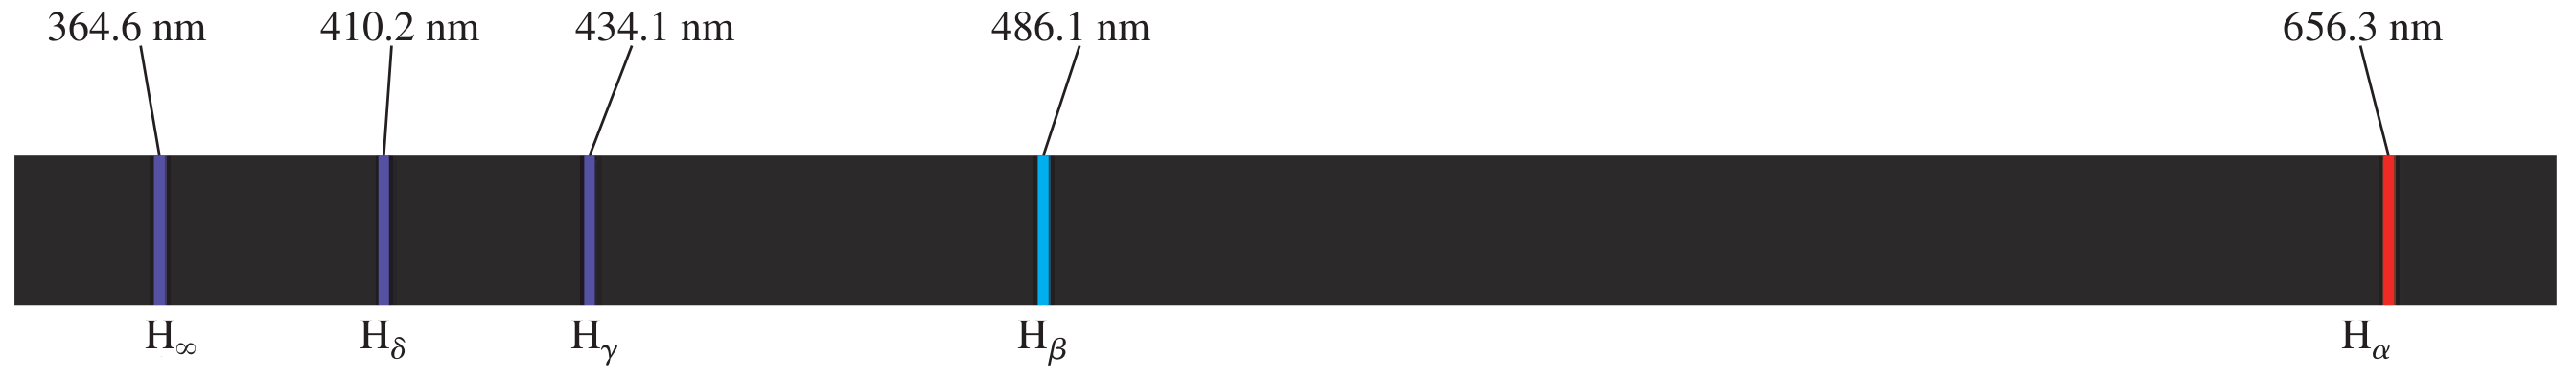
\includegraphics[width=\textwidth]{figures/H-spectrum.png}
				\caption{Serie de Balmer para el hidrógeno. Fuente: Sears \& Zemansky.}
				\label{fig:Balmer-series} 
\end{figure}

Otras series de líneas del hidrógeno son las que ocurren desde un nivel $ n >1 $ hasta el nivel $ n=1 $, que son conocidas como series de Lyman. De manera análoga, la línea debida a la transición de $ n=2 $ hasta $ n=1 $ es llamada <<Lyman alfa>> y se denota con $ \mathrm{Ly}_{\alpha} $. La transición de $ n=3 $ hasta $ n=1 $ es <<Lyman beta>>, denotada con $ \mathrm{Ly}_{\beta} $ y así sucesivamente. Las líneas de Lyman ocurren en la región ultravioleta del espectro electromagnético. Las series de Paschen corresponden a transiciones desde un nivel $ n>3 $ hasta $ n=3 $ y ocurren en la región infrarroja del espectro. La Figura \ref{fig:hidrogen-series} muestra un diagrama de la formación de líneas espectrales en el átomo de hidrógeno.

\begin{figure}[htb]
  \centering
				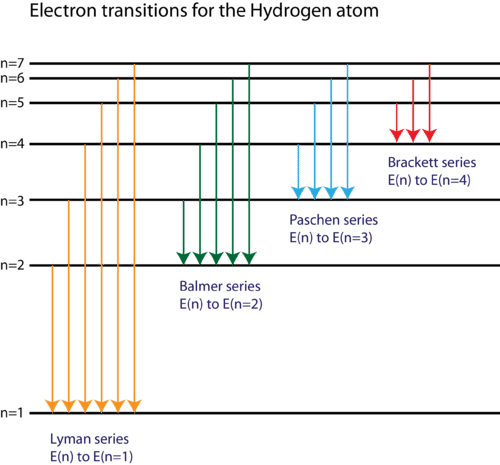
\includegraphics[width=0.8\textwidth]{figures/hydrogen-lines-transitions.png}
				\caption{Transiciones de los electrones en modelo semiclásico del átomo de hidrógeno. Fuente: \href{https://www.ck12.org/book/cbse_physics_book_class_xii/section/12.14/}{CK-12 foundation}.}
				\label{fig:hidrogen-series} 
\end{figure}

\subsubsection{Tipos de espectros}
Diferentes objetos astronómicos producen diferentes tipos de espectros. Estudiar el espectro de un objeto es uno de las formas de identificar qué tipo de objeto es. Existen tres tipos generales de espectros conocidos: (1) espectros continuos, que muestran las componentes de todos los colores del arcoíris, (2) espectros de líneas oscuras sobre un fondo brillante y (3) espectros de líneas brillantes sobre un fondo oscuro. 

En la Figura \ref{fig:types-spectra} se muestra un diagrama esquemático de cómo se producen los diferentes espectros. A continuación se explica detalladamente cada uno de ellos.

\begin{figure}[htb]
  \centering
				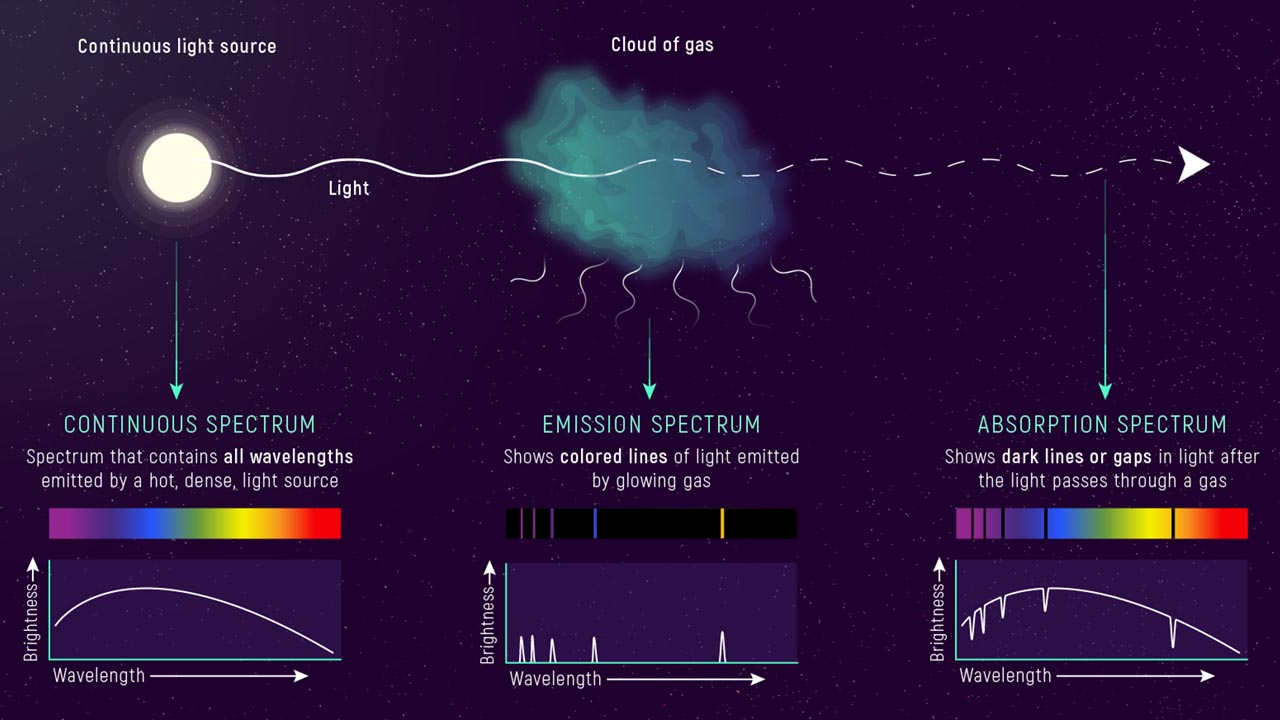
\includegraphics[width=\textwidth]{figures/types-of-spectra}
				\caption{Tipos de espectros conocidos. Fuente: \href{https://webbtelescope.org/contents/media/images/01F8GF8DK2PRY4FP9DA2XPQC8S}{Webb Space Telescope}.}
				\label{fig:types-spectra} 
\end{figure}

El \textbf{espectro continuo:} se forma a partir de objetos calientes y densos como el núcleo de las estrellas, que actúan como cuerpos negros. Si fuéramos capaces de ver la luz de estas fuentes de manera directa y sin intervención de ningún tipo de materia, entonces lo veríamos como la línea continua mostrada en el panel inferior izquierdo de la Figura \ref{fig:types-spectra}. 

El \textbf{espectro de absorción:} las estrellas están rodeadas por capas exteriores de gas que son menos densas que el núcleo. Estas capas son las atmósferas estelares. Los fotones emitidos en el núcleo abarcan todas las longitudes de onda, pero algunos con frecuencias específicas pueden ser absorbidos en la atmósfera. El efecto neto es que en la Tierra se detectan menos fotones de los generados en el núcleo y el espectro mostrará líneas de absorción que se muestran como una disminución en la intensidad, tal como aparece en el panel inferior derecho de la Figura \ref{fig:types-spectra}.

El \textbf{espectro de emisión:} ocurre cuando no se está viendo directamente a una estrella, sino a una nube de gas difusa. Los átomos de la nube pueden llevarse a estados excitados debido a su cercanía con estrellas jóvenes que emiten fotones lo suficientemente energéticos. Cuando sus átomos se desexciten, van a emitir fotones a longitudes de onda y frecuencias específicas. Debido a que la dirección en la que estos fotones son emitidos es aleatoria, un observador en la Tierra puede detectarlos y el espectro estará compuesto por líneas de emisión, como el mostrado en el panel central de la Figura \ref{fig:types-spectra}.

\subsubsection{Clasificación espectral de estrellas}
Los astrónomos han diseñado una forma bastante sencilla para diferenciar y clasificar a las estrellas de acuerdo a su temperatura efectiva, también llamada temperatura superficial. La mayoría de las estrellas están dentro de las siguientes clases espectrales: \textbf{O, B, A, F, G, K, M}. 

Las clases espectrales van desde la letra O, que son las estrellas más calientes, hasta la letra M, que son las estrellas más frías. Las letras no siguen ningún orden y pueden resultar confusas, ya que al igual que con el sistema de magnitudes, se asignaron debido a razones históricas antes que se comprendieran las propiedades físicas de las estrellas. Un método para recordar el orden de la clasificación espectral es utilizando el siguiente truco:

Oh, Be A Fine Girl, Kiss Me.

Adicionalmente, se le asigna un número entre 0 y 9 a cada letra de las clases espectrales para refinar la clasificación, de modo que los números más pequeños indican temperaturas mayores. Por ejemplo, una estrella de tipo B2 es más caliente que una de tipo B6. El Sol es una estrella de tipo G5.

\subsection{Velocidades radiales}
Una de las tareas fundamentales de la astronomía es la medición del movimiento de los objetos astronómicos. Para describir totalmente el movimiento de un objeto se necesita obtener su posición y sus componentes de velocidad en las tres coordenadas espaciales. Para describir la posición de todos los objetos se utiliza un sistema de referencia llamado <<coordenadas celestes>>, en los cuales se debe determinar su ascensión recta (RA, por sus siglas en inglés), su declinación y la dirección a lo largo de la línea de visión (LOS, por sus siglas en inglés). Para más información sobre este sistema de coordenadas puedes referirte al libro <<Fundamental Astronomy>>. 

Cuando la distancia a un objeto es conocida, las componentes de velocidad perpendiculares al LOS pueden calcularse midiendo los cambios en las coordenadas celeste con respecto al tiempo. Estas componentes de velocidad son llamadas <<\emph{movimientos propios}>> y son inversamente proporcionales a la distancia. Por lo tanto, son más fáciles de medir para objetos cercanos. La tercera componente de velocidad se mide con respecto al LOS y es llamada la velocidad radial, ya que nos indica si el objeto se acerca o se aleja de nosotros. 

Por convención en astronomía, la velocidad radial se define tal que es positiva si la distancia entre el objeto y la Tierra está incrementando (es decir, se alejan) y negativa si la distancia está disminuyendo (se acercan). Esta velocidad puede obtenerse a partir de observaciones espectroscópicas en términos del efecto Doppler.

\subsubsection{El efecto Doppler}
El efecto Doppler describe el cambio aparente en la longitud de onda (y la frecuencia) de una onda cuando existe movimiento relativo entre la fuente y el observador. El ejemplo más común es el de las ondas sonoras cuando pasa una ambulancia. 

En el contexto de las ondas electromagnéticas, se utiliza el término <<desplazamiento Doppler>> para referirse al cambio en la longitud de onda. Por ejemplo, la serie de Balmer para el hidrógeno ocurre a las longitudes de onda mostradas en la Figura \ref{fig:Balmer-series}. Si medimos el espectro de una fuente que se encuentra en reposo con respecto a la Tierra, entonces las líneas espectrales de la serie de Balmer para esa fuente serán exactamente iguales a las que se miden en el laboratorio. 

Un ejemplo más realista involucra el movimiento relativo entre una fuente astronómica y la Tierra. En este caso hay dos posible escenarios. Primero, si un objeto se mueve de tal modo que se aleja de nosotros, entonces sus líneas espectrales parecerán desplazadas hacia longitudes de onda más largas, o a la región más roja del espectro electromagnético. Este efecto recibe el nombre de <<desplazamiento al rojo>> (redshift en inglés). Mientras más rápido el objeto se aleje de nosotros, mayor será el desplazamiento al rojo. Segundo, si el objeto se mueve de modo que se acerca a nosotros, entonces sus líneas espectrales parecerán desplazadas hacia longitudes de onda más cortas, o a la región más azul del espectro. Debido a eso, este efecto se llama <<desplazamiento al azul>> (blueshift en inglés). Nuevamente, qué tan grande es el desplazamiento al azul depende de la velocidad del objeto. En la Figura \ref{fig:doppler-shift} se muestra un diagrama bastante sencillo explicando el desplazamiento Doppler. 

\begin{figure}[htb]
  \centering
				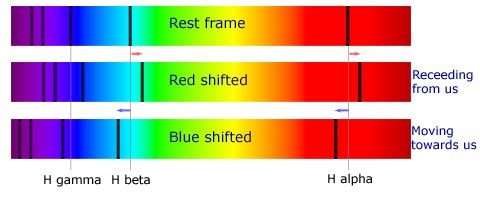
\includegraphics[width=0.7\textwidth]{figures/doppler-shift.jpg}
				\caption{Líneas espectrales de un sistema en reposo, un objeto alejándose de nosotros y otro acercándose. Fuente: \href{https://www.atnf.csiro.au/outreach//education/senior/astrophysics/spectra_info.html}{Australia Telescope National Facility (ATNF).}}
				\label{fig:doppler-shift} 
\end{figure}

Cuando una estrella o sistema astronómico se mueve con respecto a la Tierra con una velocidad radial $ v_r $ y emite un fotón a una longitud de onda $ \lambda_0 $, entonces un observador en la Tierra detectará a ese fotón con una longitud de onda desplazada debido al efecto Doppelr, $ \lambda_{\mathrm{obs}} $, donde $ \lambda_{\mathrm{obs}} \neq \lambda_0 $. El desplazamiento Doppler se obtiene realizando el cociente entre la diferencia de longitudes de onda y la longitud de onda real a la que el fotón fue emitido: $ (\lambda_{\mathrm{obs}} - \lambda_0)/\lambda_0 $. A su vez, estas dos cantidades se relacionan con la velocidad radial mediante la ecuación:
\[ \frac{\lambda_{\mathrm{obs}} - \lambda_0}{\lambda_0} = \frac{v_r}{c}, \]
donde $ v_r $ es la velocidad radial de la fuente y $ c $ es la velocidad de la luz. Si la fuente se acerca a nosotros, entonces $\lambda_{\mathrm{obs}}$ se desplaza hacia el azul y es menor que $\lambda_0$ y por lo tanto $v_r$ es negativa. En cambio, si la fuente se aleja de nosotros, $\lambda_{\mathrm{obs}}$ se desplaza hacia el rojo y es mayor que $\lambda_0$ y $v_r$ es positiva. Una de sus aplicaciones es el estudio de sistemas binarios donde la única información que tenemos son sus líneas de emisión o absorción. 

\subsubsection{Sistemas binarios espectroscópicos}
Este tipo de sistemas binarios se caracteriza porque están muy lejos y sus componentes estelares no pueden resolverse incluso con los telescopios más grandes. Sin embargo, es posible obtener información sobre el sistema gracias al análisis de su espectro. En realidad, la mayoría de los sistemas binarios detectados son gracias al desplazamiento Doppler y la espectroscopía.

La Figura \ref{fig:spectroscopic-binary} muestra una representación esquemática de un sistema binario espectroscópico. La elipse de color azul representa la órbita de la estrella $A$, mientras que la elipse de color negro representa la órbita de la estrella $B$. El punto rojo representa el centro de masa alrededor del que ambas estrellas orbitan. La dirección hacia la Tierra es hacia abajo. En la etapa 1, la estrella $A$ se encuentra en un punto de la órbita en la que se mueve en dirección a la Tierra, por lo tanto, al revisar su espectro se observa que está desplazado hacia el azul. Al mismo tiempo, la estrella $B$​​ se encuentra en un punto de su órbita en la que se mueve alejándose de la Tierra, por lo tanto, su espectro está desplazado hacia el rojo.

\begin{figure}[htb]
  \centering
				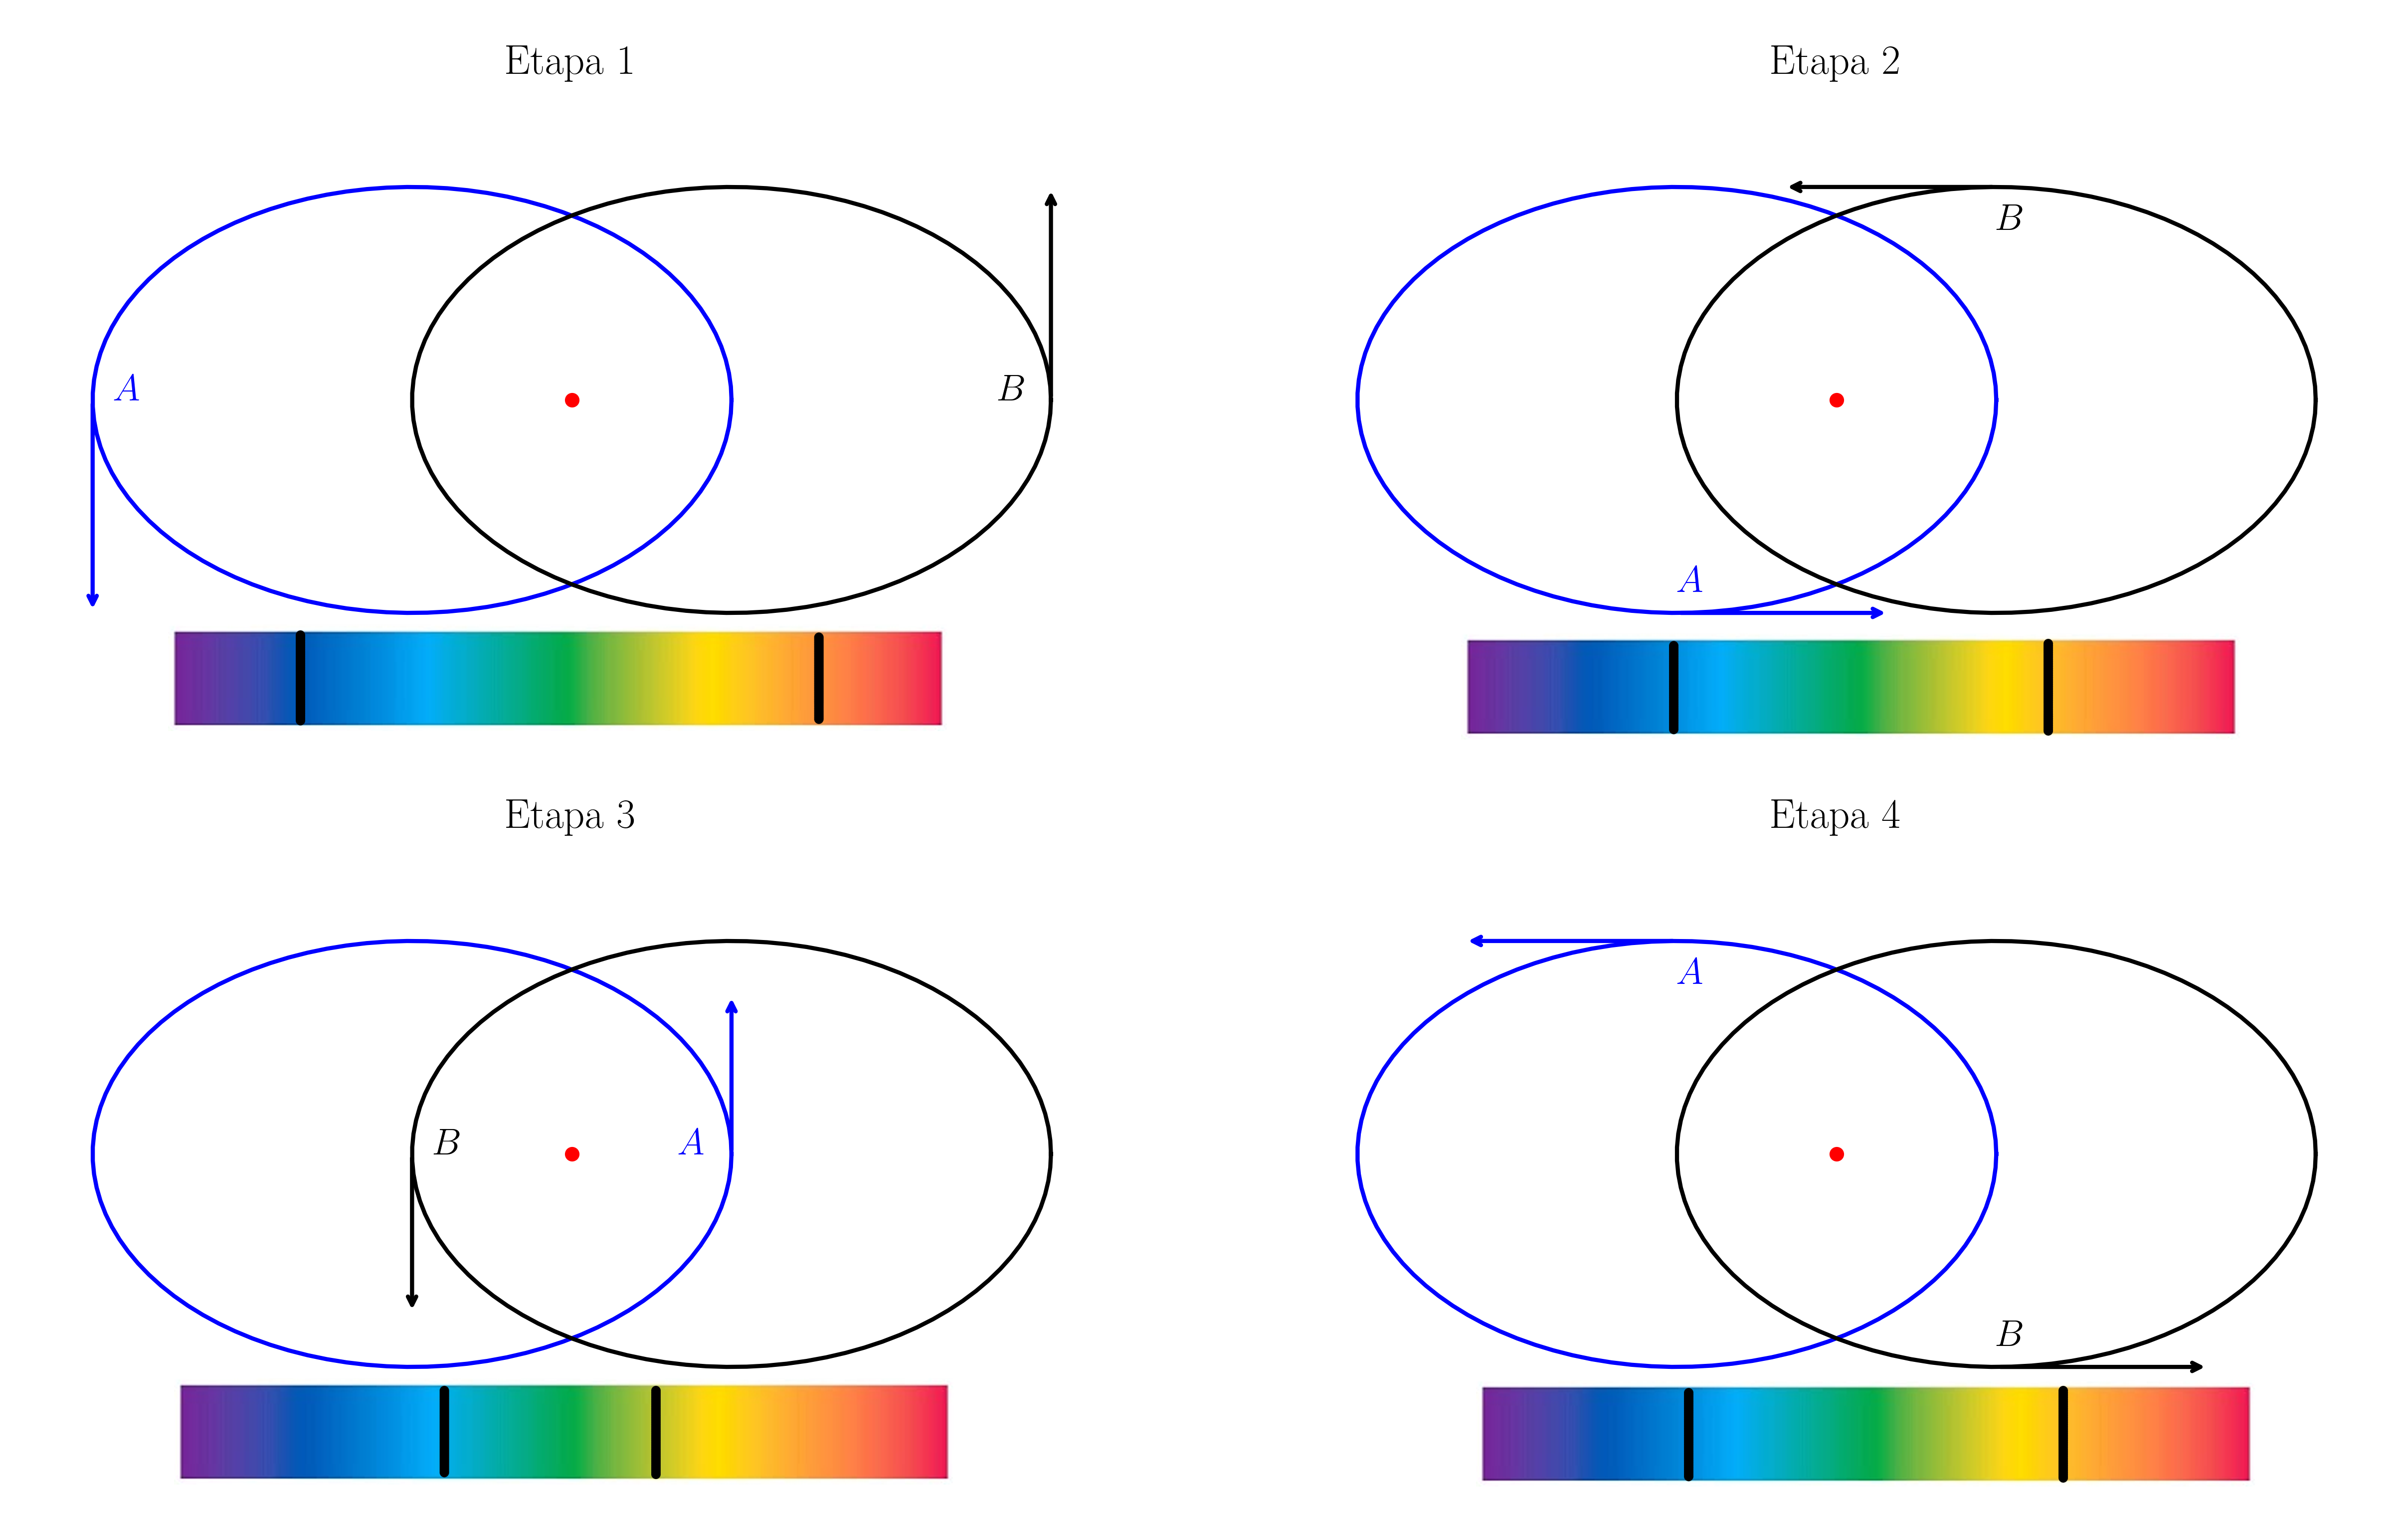
\includegraphics[width=\textwidth]{figures/Orbits-binary.png}
				\caption{Esquema de las líneas espectrales observadas en un sistema binario espectrscópico.}
				\label{fig:spectroscopic-binary} 
\end{figure}

En la etapa 2, ambas se estrellas se encuentran en una posición en su órbita donde no parece que se alejen ni que se acerquen a la Tierra. Su espectro no se ve afectado por el efecto Doppler. En la etapa 3, la situación es opuesta a la etapa 1: la estrella $A$ parece alejarse y su espectro está desplazado hacia el rojo, mientras que la estrella $B$ parece acercarse y su espectro está desplazado hacia el azul. En la etapa 4, la situación es similar a la etapa 2 y el espectro no se ve afectado por el efecto Doppler.

Ya que la velocidad radial de las estrellas puede calcularse con el efecto Doppler, es posible construir una gráfica de cómo varía la velocidad con respecto al tiempo. Dicha curva de luz se muestra en la Figura \ref{fig:lc-scb}, donde se observa un comportamiento periódico. Estas son características únicas de los sistemas binarios y gracias a la espectroscopía es posible detectarlos aún cuando se encuentran demasiado lejos para ser vistos por telescopios.

\begin{figure}[htb]
  \centering
				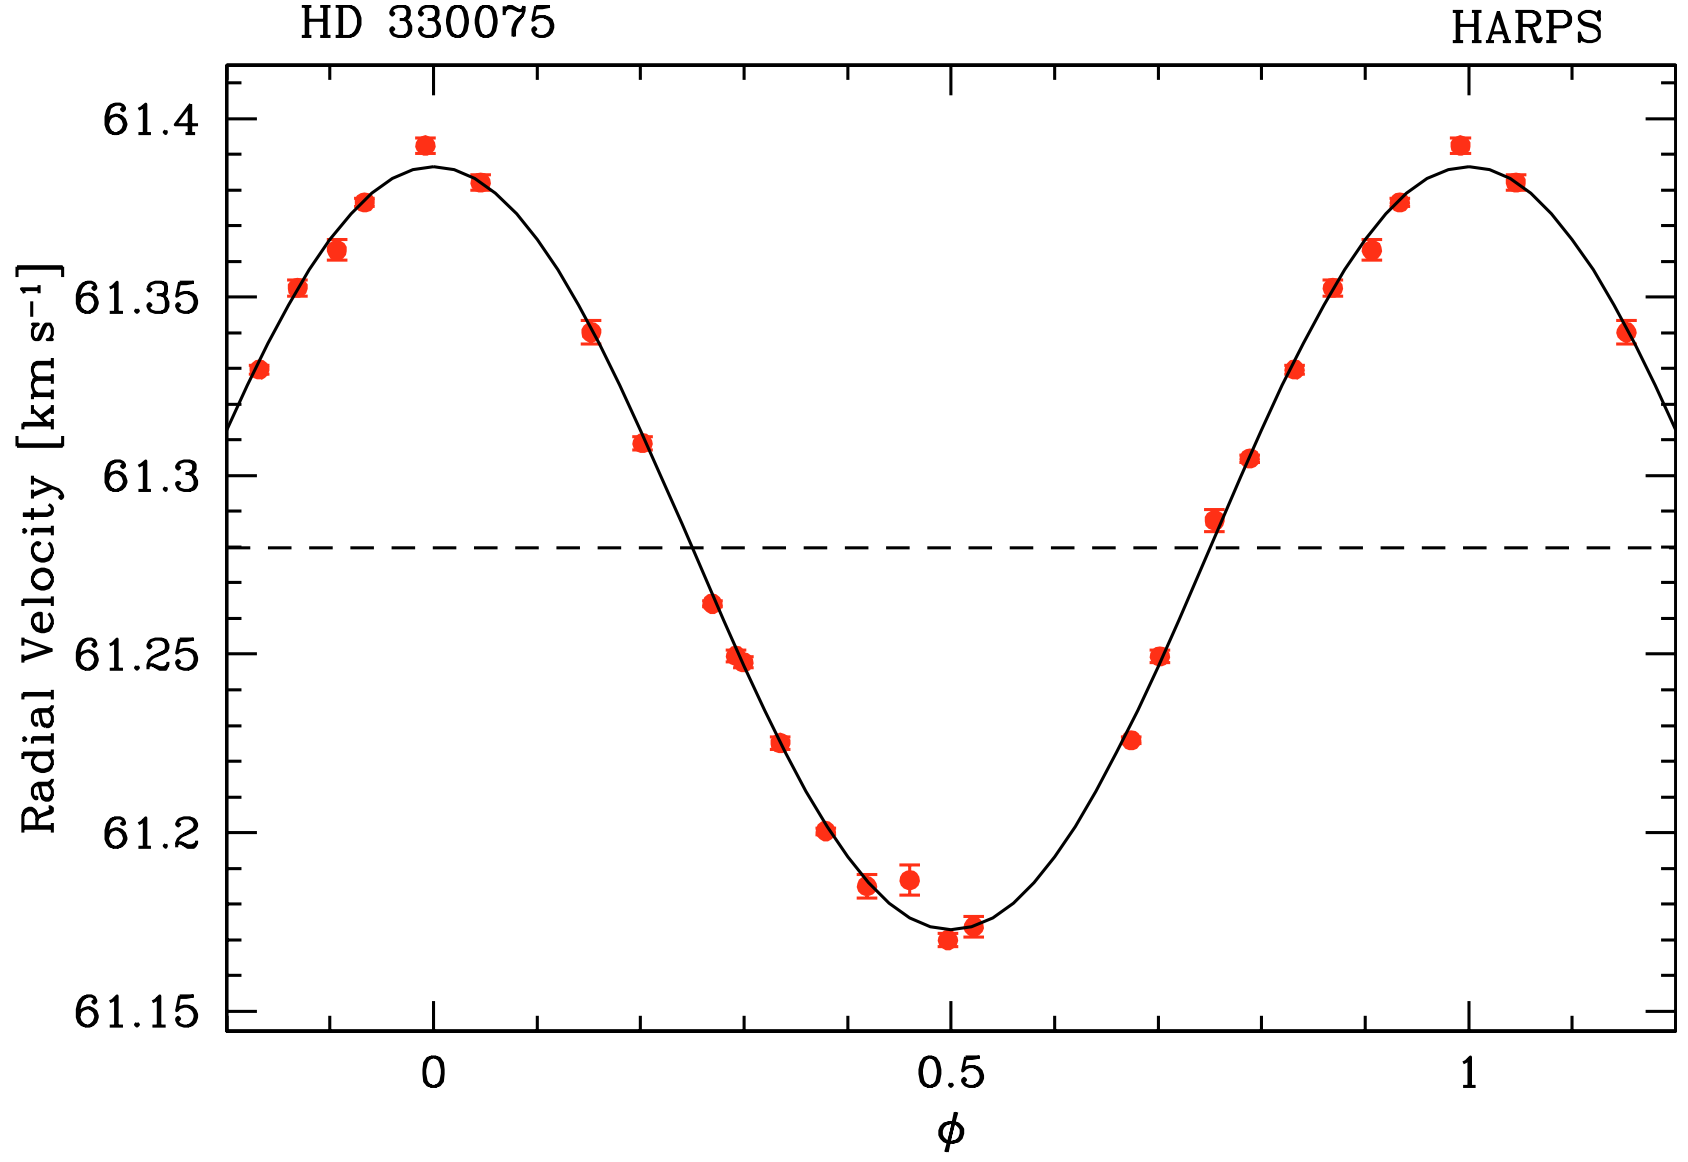
\includegraphics[width=\textwidth]{figures/spectroscopic-binary-lc.png}
				\caption{Curva de velocidad radial para el sistema binario HD 330075 tomado con el espectrógrafo <<High-Accuracy Radial-velocity Planet
Searcher>> (HARPS). Fuente: \href{https://www.aanda.org/articles/aa/abs/2004/31/aa0389-04/aa0389-04.html}{Pepe et al (2004).}}
				\label{fig:lc-scb} 
\end{figure}
